% mainfile: ../../main.tex
\chapter{Vibration performance}\label{ch:setup:vibrations}
\AutoLettrine{Noise}

\section{Accelerometric vibration spectroscopy}\label{sec:setup:vibrations:accel}

\begin{figure}
    \centering
    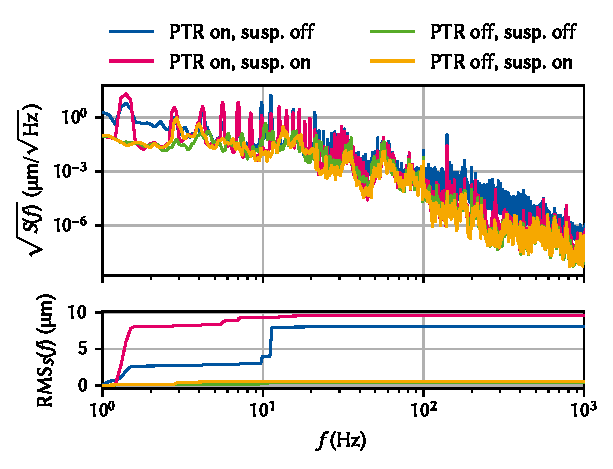
\includegraphics{pdf/setup/spect_accel}
    \caption{}
    \label{fig:}
\end{figure}

\section{Optical vibration spectroscopy}\label{sec:setup:vibrations:optic}

\begin{marginfigure}
    \centering
    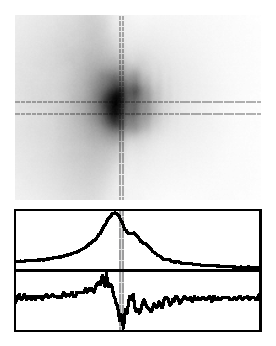
\includegraphics{pdf/setup/knife_edge}
    \caption{}
    \label{fig:}
\end{marginfigure}

\begin{marginfigure}
    \centering
    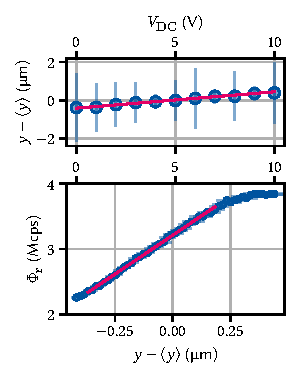
\includegraphics{pdf/setup/knife_edge_fits}
    \caption{}
    \label{fig:}
\end{marginfigure}

\begin{marginfigure}
    \centering
    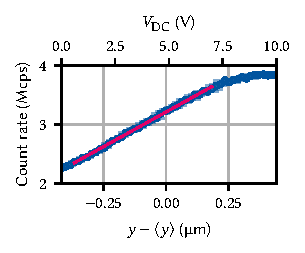
\includegraphics{pdf/setup/knife_edge_slope}
    \caption{}
    \label{fig:}
\end{marginfigure}

\begin{figure}
    \centering
    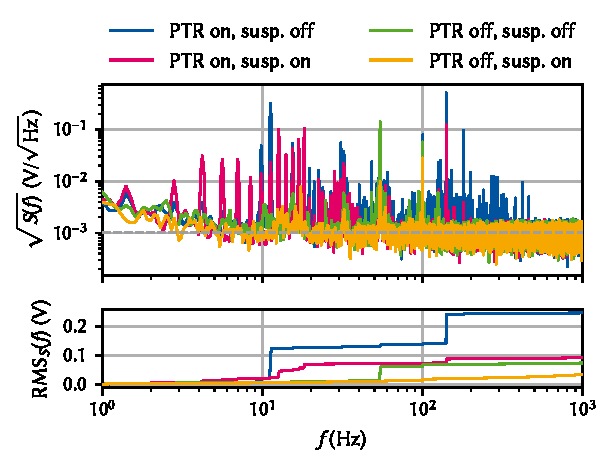
\includegraphics{pdf/setup/spect_optic}
    \caption{}
    \label{fig:}
\end{figure}
